\documentclass[10pt]{article}


% Tous les packages prédéfinis
\usepackage{introLatex}
\usepackage{headfootLatex}
\usepackage{shortcutLatex}
\usepackage{envLatex}
\usepackage{booktabs}
\graphicspath{{logos/}{figures/}}


\makeatletter
\def\hlinewd#1{%
\noalign{\ifnum0=`}\fi\hrule \@height #1 %
\futurelet\reserved@a\@xhline}
\makeatother


\begin{document}


% Titre du document
\begin{center}
\textbf{\Large Méthode multipole rapide pour un nuage de points}\\
\vspace*{4pt}
Gaétan Facchinetti \\
{\small 5 décembre 2016\\
\vspace*{5pt}
\textit{Université Paris-Saclay}, \textit{Ecole Normale Supérieure de Cachan}}, \\
\textit{Ecole Nationale Supérieure des Techniques Avancées}\\
\end{center}

\vspace*{22pt}


\begin{multicols}{2}



\section*{Question 1}

Nous avons créer une fonction permettant de renvoyer, pour une densité de point par longueur d'ondre $n_\lambda$ et une fréquence $f$ donnée, un tableau de coordonnées de l'ensemble des points du nuages ainsi que le nombre de $N$ points. Dans notre code ce nombre de points se calcule en fonction des paramètres par la formule, 

\begin{equation}
N = 4s_a(s_b-1) + 2(s_b-2)^{2}
\label{eq:N}
\end{equation}

Avec $s_a = \mathbb{E}(f n_\lambda L/c)+1$ et $s_b = \mathbb{E}(f n_\lambda l/c)+1$, où $L=1$ (m) et $l=0.5$ (m) sont les dimensions de la boite et $c$ la célérité de l'onde dans le milieu considéré Nous avons alors pu représenter en \refig{Q1} les points de discrétisation.


\begin{figure}[H]
  \begin{center}
  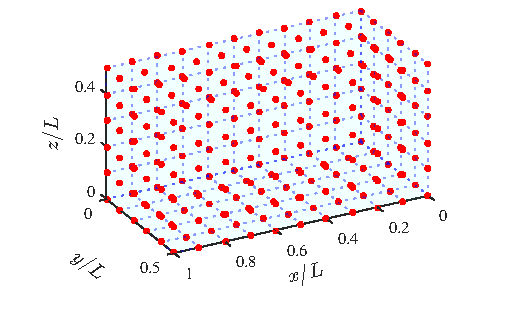
\includegraphics[width=0.95\columnwidth]{Q1_4.pdf}
  \vspace*{-11pt}
  \caption{Points de discrétisation suivant les trois coordonnées spatiales (rouge). $N=252$, $n_\lambda = 10$, $f = c/L$. Pour faciliter la lecture les plans $x=0$, $y=0$ et $z=0$ ont été représentés en cyan.}
  \label{fig:Q1}
  \end{center}
\end{figure}
\vspace*{-22pt}


\vspace*{22pt}



\section*{Question 2}

Notons, pour $i \in \bbrac{1,N}$, $\xv_i$ le vecteur position du point du nuage indicé $i$. Introduisons alors la matrice de la fonction de Green G que nous definissons par :

\begin{equation}
\forall (i,j) \in \bbrac{1,N}^{2} \quad G_{i,j} =
 \begin{cases}
   \frac{e^{ik\lb \xv_i - \xv_j \rb}}{\lb \xv_i - \xv_j \rb} & \text{si } i\neq j \\
   0 & \text{si } i=j
 \end{cases}
\end{equation}


Nous notons $\tau_{a}$ le temps d'assemblage de cette matrice. Soit maintenant un vecteur $\rhov$ quelconque de $\R^{N}$. Nous notons $\tau_c$ le temps de calcul du produit matrice vecteur $\Vv = G\rhov$.\\

Nous pouvons remarquer qu'à partir de $N \sim 10 000$ l'assemblade de la matrice est trop gourmand en mémoire et cela rend l'execution sous Matlab impossible. Nous avons donc fait varier $n_\lambda$ à $f$ fixé pour avoir, d'après \refeq{N}, une valeur de $N$ maximale de 9002. Puis nous avons représenté en \refig{Q2a} et \refig{Q2b} l'évolution de $\tau_a$ et $\tau_c$ en fonction de $N$.



\begin{figure}[H]
  \begin{center}
  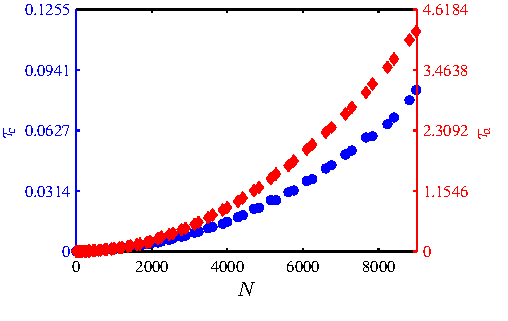
\includegraphics[width=0.95\columnwidth]{Q2a_4.pdf}
  \vspace*{-11pt}
  \caption{Temps d'assemblage de $G$, $\tau_a$ (losanges rouge) et temps de calcul du produit matrice vecteurs $\tau_c$ (ronds bleu) en fonction de $N$. Les deux courbes ont une allure parabolique mais nous pouvons remarquer que, les echelles étant différentes, le temps d'assemblage est plus long}
  \label{fig:Q2a}
  \end{center}
\end{figure}
\vspace*{-22pt}

\begin{figure}[H]
  \begin{center}
  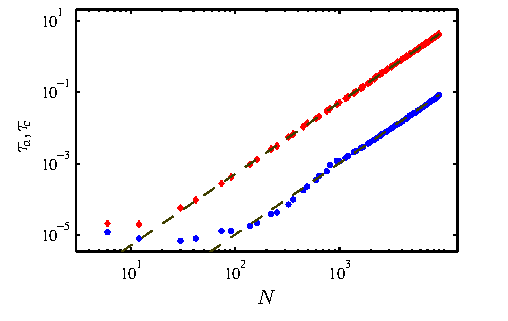
\includegraphics[width=0.95\columnwidth]{Q2b_4.pdf}
  \vspace*{-11pt}
  \caption{Temps d'assemblage de $G$, $\tau_a$ (losanges rouge) et temps de calcul du produit matrice vecteurs $\tau_c$  (ronds bleu) en fonction de $N$. Nous pouvons remarquer ici qu'asymptotiquement $\log(\tau_{a/c}) \simeq 2\log(N)+K_{a/c}$ représentées en pointillé vert avec $K_{a/c}$ constante.}
  \label{fig:Q2b} 
  \end{center}
\end{figure}
\vspace*{-22pt}

Comme il l'est montré en \refig{Q2b}, l'évolution du logarithme de $\tau_a$ avec $N$ tend asymptotiquement vers une droite de pente 2. Il est en cd même pour le logarithme de $\tau_c$ avec $N$. Ceci confirme l'évolution en $O(N^{2})$ du temps d'assemblage et de produit matrice vecteur.



\vspace*{22pt}

\section*{Question 3}

Nous avons calculé la quadrature de Gauss-Legendre à L points en diagonsalisant la matrice tridiagonale définie dans l'énoncé. La methode utiliséé pour obtenir les points de quadrature est la méthode de Golub-Welsh\footnote{\textit{Calculation of Gauss Quadrature Rules}, G.H. Golub and J.H. Welsh \color{cyan}, Math. Comp. 23 (1969), 221-230 \color{black}, (Apr., 1969)}. Avec les notations du TP nous calculons, pour P polynôme tel que $\text{deg}P \le 2L-1$,

\begin{equation}
	\int_{-1}^{1}{P(t)dt} = \sum_{i=1}^{L}{\omega_i P(\lambda_i)}
\end{equation}

Ceci est équivalent, par un changement de variable, à

\begin{equation}
	\int_{0}^{\pi}{P(\cos(t))\sin(t)dt} = \sum_{i=1}^{L}{\omega_i P(\cos(\theta_i))}
\end{equation}

Nous avons testé cette quadrature avec $L = 3$ en comparaison de celle à 3 points dévleoppée lors du premier TP. Nous écrivons $I_{GL}$ le résultat par la quadrature de Gauss Legendre, $I_{1}$ le résultat pour la quadrature à trois points du premier TP, $I_{M}$ le résultat de la qudrature effectuée par Matlab et $I_v$ la valeur vraie pour l'integration de la fonction polynomiale $P$.

\begin{table}[H]
\centering
\begin{tabular}{m{2cm} |m{1cm} m{1cm} m{1cm} m{1cm}} 
   \hline
    \centering $P$ & $I_{GL}$ & $I_{1}$ & $I_{M}$ & $I_v$ \\
    \toprule
    \toprule
    $x \mapsto x$      & 0.00 & 0.00 & 0.00 & 0 \\
    $x \mapsto x^{2}$  & 0.667 & 0.667 & 0.667 & 2/3 \\
    $x \mapsto x^{4}$  & 0.400 & 0.667 & 0.400 & 2/5 \\
    \hline
\end{tabular}
\caption{Résultat des quadratures numériques}
\end{table}

Comme attendu nous observons que pour la quadrature de Gauss-Legendre donne les même resultats pour des polynômes de degré inférieur ou égal à 3 que la quadrature du premier TP. En revanche, comme nous pouvions nous y attendre cette nouvelle quadrature nous permet d'avoir une solution correcte pour des polynomes de degré 4 et 5, puisque la formule est bien exacte jusqu'au degé $2L-1$.


\vspace*{12pt}

\section*{Question 4}

Notons 
\begin{equation}
	C_{l,m} = \sqrt{\frac{2l+1}{4\pi}\frac{(l-m)!}{(l+m)!}}
\end{equation}

Nous avons, par définition, 
\begin{equation}
Y_{lm}(\theta, \phi) = C_{l,m}P_l^{m}\(\cos(\theta)\)e^{im\phi}
\end{equation}

En notant $I$ l'intégrale de $Y_{lm}$ sur la sphère unité, 
\begin{equation}
I = C_{l,m}\int_{0}^{\pi}{P_l^{m}\(\cos(\theta)\)\sin(\theta)d\theta}\int_{0}^{2\pi}e^{im\phi}d\phi
\end{equation}

Ainsi si $m \neq 0$ l'integrale sur $\phi$ donne directement $I = 0$.  De plus, d'après d'autres propriétés des polynomes de Legendre, la quadrature totale doit alors satisfaire les égalités suivantes :
\begin{equation}
\sum_{i,j}{\omega_i \omega_j Y_{lm}(\theta_j, \phi_i)} = 
	\begin{cases}
		0 & \text{ si } m \neq 0 \text{ et } l \neq 0 \\
		\sqrt{4\pi} & \text{ si } m = 0 \text{ ou } l = 0
	\end{cases}
\end{equation}

En particulier, la quadrature sur $\phi$ doit vérifier : 
\begin{equation}
	\sum_{i}{\omega_i e^{im\phi_i}} = 
	\begin{cases}
		0 & \text{ si } m \neq 0 \\
		2\pi & \text{ si } m = 0 \\
	\end{cases}
\end{equation}

L'avantage de cette quadrature ...

\vspace*{22pt}

\section*{Question 5}

\subsection*{Mise en pratique}

Nous souhaitons calculer la décomposition en onde plane de la fonction de green G. Posons $\xv - \yv = (\yv_0 - \yv) + (\xv_0 - \yv_0) - (\xv_0 - \xv) = \rv + \rv_0$. Nous utilisons les formules 

\begin{equation}
	G(\xv, \yv) = \frac{\exp(ik|\xv-\yv|)}{|\xv-\yv|} \simeq \int_{S^{2}}{e^{ik\svh\rv}\Gc_Ld\svh}
\end{equation}

\vspace*{-22pt}

\begin{equation}
\Gc_L = \frac{ik}{4\pi}\sum_{p=0}^{L}{(2p+1)i^{p}h_p^{(1)}(k|\rv_0|)P_p(\cos(\svh, \rv_0))}
\end{equation}
\begin{equation}
\cos(\svh, \rv_0) = \frac{1}{|\rv_0|}< \begin{pmatrix} \sin(\theta)\cos(\phi)  \\ \sin(\theta)\sin(\phi)  \\ \cos(\theta) \end{pmatrix} , \rv_0 >
\end{equation}


L'intégrale sur la sphére unité est alors calculée par la quadrature à $(2L+1)(L+1)$ points déterminée dans la question précédente. Attention cependant car il ne faut pas prendre les fonctions de Hankel \textit{besselh} telles que définies sous Matlab car cela ne donne pas les bons résultats. En effet nous devons utiliser pour nos formules, pour $(z,p) \in \R^{*}_{+}\times\N$ 

\begin{equation}
	h^{(1)}_{p}(z) = e^{iz}\sum_{k=0}^{p}{\frac{(p+k)!}{2^{k}(p-k)!}\frac{1}{z^{k+1}}}
\end{equation}

Pour être plus rapide dans le code ces fonctions sont en réalité calculées à l'aide de la formule de récurrence 

\begin{equation}
	h_{p+1}^{(1)}(z) =  \frac{2p+1}{z}h_{p}^{(1)}(z) - h_{p-1}^{(1)}(z) 
\end{equation}


\vspace*{10pt}


\subsection*{Un exemple de cas test}

Pour tester nos codes nous avons utilisé le cas test $\rv = 0$ et $\rv_0 = \xv - \yv$. En effet dans ce cas nous pouvons écrire

\begin{equation}
G(\xv,\yv) = {\sum_{p=0}^{L}{\frac{(2p+1)k}{4\pi}i^{p+1}h_p^{(1)}(k|\rv_0|)\int_{S^{2}}P_p(\cos(\svh, \rv_0))}d\svh}
\end{equation}

Cependant pour $p\in\bbrac{0,L}$ comme notre quadrature intègre exactement les polynomes de degrés inférieur ou égal à $2L+1$ et d'après l'ortogonalité des polynômes de Legendre, il vient, 

\begin{equation}
G(\xv,\yv) = ikh^{(1)}_{p}(k|\rv_0|)
\end{equation}

Ceci nous permet alors de confirmer le choix des fonctions de Hankel et le bon fonctionnement de la quadrature sur les polynômes de Legendre.



\vspace*{10pt}

\subsection*{Resultats}

Nous avons donc un code qui fonctionne bien sur le cas test précédemment. De plus ... 


\end{multicols}




\end{document}
